% Bab 1  Pendahuluan
\chapter{PENDAHULUAN}

\section{Latar Belakang}
Latar belakang masalah harus menjelaskan rumusan masalah yang akan dibahas dan dicarikan penyelesaiannya. Selain itu, latar belakang masalah juga harus dapat menjelaskan mengapa topik penelitian yang dilakukan dipandang menarik, penting, dan layak untuk diteliti. Berikan data pendukung yang memadai untuk meyakinkan pembaca bahwa penelitian yang Penulis lakukan penting.

Dokumen ini adalah \textit{template} proposal skripsi yang resmi dikeluarkan oleh Rekayasa Sistem Komputer Universitas Muhammadiyah Buton (UM Buton). Dokumen proposal skripsi harus dibuat pada kertas A4 dengan \textit{margin} atas, kanan, bawah, dan kiri secara berurutan adalah 4 cm, 3 cm, 3 cm, dan 4 cm. Format penulisan proposal skripsi adalah \textit{Times New Roman} dengan ukuran \textit{text} 12 pt dan berspasi 1,5 \textit{lines}. Jelaskan penggunaan singkatan dan akronim saat pertama kali muncul. Untuk hitungan yang memiliki angka desimal, gunakan tanda koma (“,”) untuk memisahkan pecahan desimal tersebut, contoh: “0,25; 7,56; …”.

Contoh kalimat bersitasi: Penjadwalan paket pada jaringan seluler berperan penting dalam membagi sumber daya radio secara adil di antara pengguna (Capozzi et al., 2013). Andrews (2007) menyatakan bahwa teori penjadwalan pada jaringan data nirkabel terus berkembang seiring bertambahnya kebutuhan layanan. Kebutuhan serupa juga muncul pada jaringan listrik cerdas yang menuntut penjadwalan waktu nyata (Xu \& Fischione, 2012). Data statistik nasional dipublikasikan secara berkala oleh lembaga resmi (Badan Pusat Statistik, 1997).

\section{Rumusan Masalah}
Rumusan masalah disusun berdasarkan latar belakang, berbentuk pertanyaan penelitian atau pernyataan yang memerlukan jawaban melalui penelitian ilmiah, dan ditulis dalam bentuk butir bernomor:
\begin{enumerate}
\item Bagaimana ... ?
\item Seberapa besar ... ?
\end{enumerate}

\section{Tujuan Penelitian}
Tujuan penelitian dinyatakan dalam kalimat singkat, jelas, dan spesifik, serta konsisten dengan rumusan masalah (satu tujuan untuk satu rumusan masalah):
\begin{enumerate}
\item Merancang ...
\item Mengukur ...
\end{enumerate}

Keterkaitan rumusan masalah, tujuan, dan indikator keberhasilan dapat diringkas dalam tabel, seperti pada Tabel 1.1 (data contoh).

\begin{singlespace}
\begin{longtable}{|c|p{0.28\linewidth}|p{0.28\linewidth}|p{0.22\linewidth}|}
\caption{Contoh keterkaitan rumusan masalah, tujuan, dan indikator keberhasilan}\\
\hline
\textbf{No.} & \textbf{Rumusan masalah} & \textbf{Tujuan} & \textbf{Indikator} \\
\hline
1 & Bagaimana merancang sistem pemantauan suhu berbasis ESP32? & Merancang sistem pemantauan suhu berbasis ESP32 & Sistem berfungsi pada 10 kali uji \\
\hline
2 & Seberapa besar akurasi sensor suhu yang digunakan? & Mengukur akurasi sensor suhu & Galat rata-rata $\leq$ 2\% \\
\hline
\end{longtable}
\end{singlespace}

\section{Manfaat Penelitian}
Tulis manfaat penelitian yang ingin Penulis capai. Ruang lingkup sistem yang akan dikembangkan dapat diperjelas dengan gambar, seperti Gambar 1.1 (sketsa contoh).

Contoh kalimat bersitasi: Perangkat keras yang digunakan mengikuti spesifikasi dari pabrikan (Espressif Systems, 2023).

\begin{figure}[H]
\centering
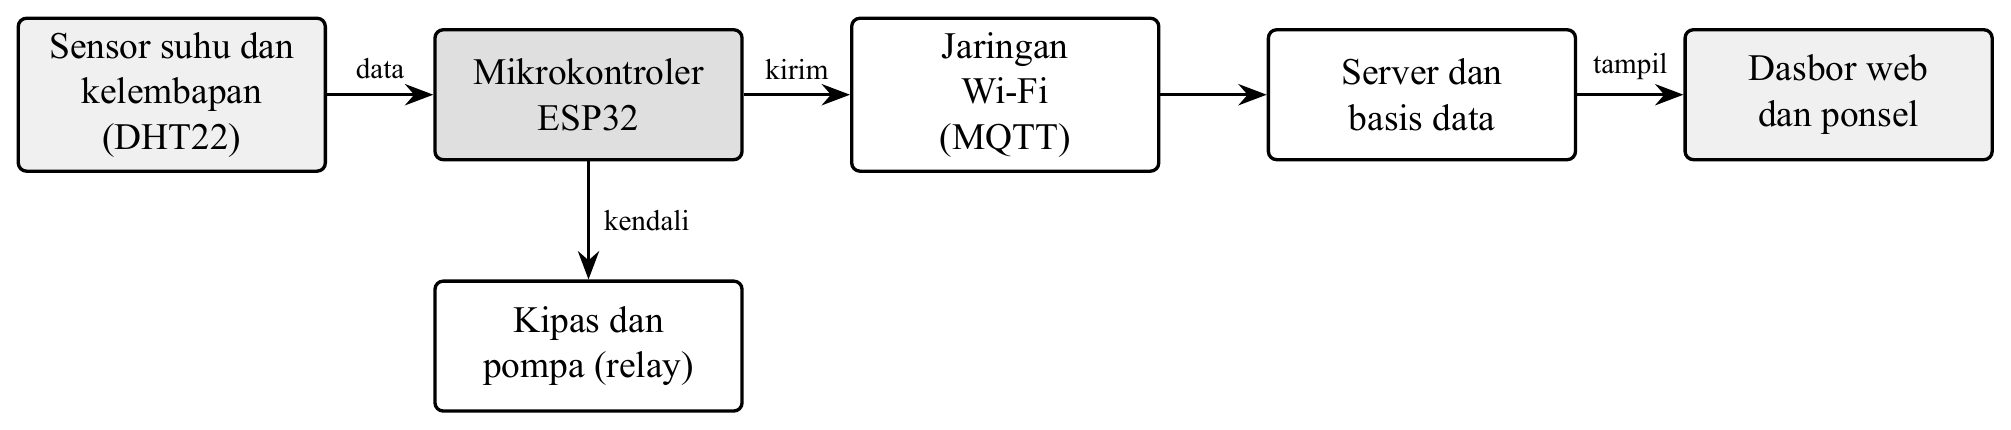
\includegraphics[width=\textwidth]{../00-gambar/contoh-sistem.png}
\caption{Contoh gambaran umum sistem yang akan dikembangkan}
\end{figure}

